\documentclass[12pt]{article}
        \makeatletter
        \def\input@path{{../../}}
        \makeatother
        \usepackage{sbc-template}
        \makeatletter
        \renewcommand{\inst}[1]{}
        \makeatother
        \usepackage{graphicx,url}
        \usepackage[utf8]{inputenc}
        \usepackage[T1]{fontenc}
        \usepackage[brazil]{babel}
        \usepackage{longtable,booktabs,array}
        \usepackage{amsmath,amssymb}
        \providecommand{\tightlist}{%%
          \setlength{\itemsep}{0pt}\setlength{\parskip}{0pt}}
        \sloppy
        \title{Quantum Reservoir Computing para previsão de demanda: um estudo didático com o Favorita}
        \author{}
        \address{}
        \begin{document}

        \maketitle

        \begin{resumo}
        Este artigo fecha a série com um estudo completo e didático de Quantum Reservoir Computing (QRC) aplicado ao recorte adotado no Favorita desde o primeiro capítulo. O texto unifica tudo o que foi construído anteriormente: problema de negócio, protocolo experimental, benchmark justo, intuição de reservatório e ponte conceitual para o quântico. Em seguida, apresenta o pipeline do QRC implementado com Qiskit, compara as configurações \texttt{14x7} e \texttt{8x5}, discute a função objetivo usada no tuning e posiciona os resultados do QRC ao lado de \texttt{ETS}, \texttt{XGBoost} e \texttt{RC}. O resultado final é instrutivo: o QRC funciona de ponta a ponta, \texttt{14x7} e a melhor configuração por desempenho puro, \texttt{8x5} e o melhor compromisso pela função objetivo, mas as técnicas clássicas seguem superiores neste recorte.
        \end{resumo}

        \subsection{1. O que o leitor vai aprender}\label{1-o-que-o-leitor-vai-aprender}

Ao final deste artigo, você será capaz de:

\begin{enumerate}
\def\labelenumi{\arabic{enumi}.}
\tightlist
\item
  descrever o pipeline completo de QRC do projeto;
\item
  executar o modelo com Qiskit no recorte adotado no Favorita;
\item
  interpretar por que \texttt{14x7} e \texttt{8x5} coexistem como candidatos fortes;
\item
  comparar o QRC com RC e modelos clássicos no mesmo protocolo;
\item
  concluir o que a série inteira ensina sobre a rota até QRC.
\end{enumerate}

\subsection{2. O recorte experimental herdado da série}\label{2-o-recorte-experimental-herdado-da-suxe9rie}

O estudo final não muda o problema para favorecer o QRC. Ele preserva:

\begin{itemize}
\tightlist
\item
  \texttt{store\_nbr\ =\ 1}
\item
  \texttt{family\ =\ BEVERAGES}
\item
  frequência diária
\item
  últimos \texttt{90} dias como teste
\end{itemize}

Isso garante continuidade didática e comparabilidade científica.

\subsection{3. Pipeline de QRC usado no projeto}\label{3-pipeline-de-qrc-usado-no-projeto}

\subsubsection{3.1 Entrada}\label{31-entrada}

O QRC usa um vetor de entrada clássico reduzido:

\[
u_t =
\begin{bmatrix}
\widetilde{y}_{t-1} &
\widetilde{p}_t &
\sin(2\pi \, \mathrm{dow}_t / 7) &
\cos(2\pi \, \mathrm{dow}_t / 7)
\end{bmatrix}^\top.
\]

Essa reducao aparece em \texttt{\_quantum\_input\_vector()}, que seleciona os quatro primeiros componentes do vetor sequencial clássico.

\subsubsection{3.2 Dinâmica quântica}\label{32-dinuxe2mica-quuxe2ntica}

Para cada passo da janela, o circuito aplica rotações \texttt{RX} e \texttt{RY} em todos os qubits e um anel de emaranhamento \texttt{CZ} + \texttt{RZ}. Se chamarmos o operador de um passo de \(U(u_t)\), a representação da janela fica

\[
|\psi_t\rangle = U(u_t) U(u_{t-1}) \cdots U(u_{t-w+1}) |0 \cdots 0\rangle.
\]

\subsubsection{3.3 Observáveis}\label{33-observuxe1veis}

As features quânticas sao expectativas:

\[
z_t^{(j)} = \langle \psi_t | O_j | \psi_t \rangle.
\]

O projeto usa observáveis \texttt{Z}, \texttt{X} e \texttt{ZZ}, totalizando \texttt{3q} componentes para \texttt{q} qubits.

\subsubsection{3.4 Readout}\label{34-readout}

O readout final continua sendo simples:

\[
\hat{y}_t = W_{out} [1; u_t; z_t],
\]

com treinamento Ridge:

\[
W_{out}^* = \arg\min_{W_{out}} \|Y - \Phi W_{out}\|_2^2 + \lambda \|W_{out}\|_2^2.
\]

Em outras palavras, o QRC do projeto herda a filosofia central de RC: dinâmica rica, readout simples.

\subsection{4. Implementação passo-a-passo}\label{4-implementauxe7uxe3o-passo-a-passo}

O leitor pode percorrer a implementação nesta ordem.

\subsubsection{4.1 Passo 1: definir a configuração}\label{41-passo-1-definir-a-configurauxe7uxe3o}

\begin{verbatim}
@dataclass(frozen=True)
class QRCConfig:
    n_qubits: int = 14
    window: int = 7
    input_scale: float = 1.2
    ridge_alpha: float = 1e-1
    seed: int = 7
\end{verbatim}

\subsubsection{4.2 Passo 2: construir o circuito por passo}\label{42-passo-2-construir-o-circuito-por-passo}

O código central esta em \texttt{\_step\_circuit()} e usa \texttt{QuantumCircuit} do Qiskit.

\subsubsection{4.3 Passo 3: acumular a janela quântica}\label{43-passo-3-acumular-a-janela-quuxe2ntica}

\texttt{features\_from\_window()} compoe sucessivos passos do circuito antes de criar o \texttt{Statevector}.

\subsubsection{4.4 Passo 4: medir observáveis}\label{44-passo-4-medir-observuxe1veis}

O método \texttt{\_build\_observables()} cria as listas de operadores \texttt{Z}, \texttt{X} e \texttt{ZZ}.

\subsubsection{4.5 Passo 5: ajustar o readout e prever}\label{45-passo-5-ajustar-o-readout-e-prever}

\texttt{fit\_qrc\_readout()} treina o Ridge e \texttt{forecast\_qrc()} faz previsão recursiva no bloco de teste.

Para executar:

\begin{verbatim}
python code/qrc/run.py
pytest code/qrc/test_model.py
pytest code/qrc/test_objective.py
\end{verbatim}

\subsection{5. Configuração experimental}\label{5-configurauxe7uxe3o-experimental}

O tuning anterior deixou duas configurações principais:

\begin{itemize}
\tightlist
\item
  melhor configuração por rank médio multi-métrica: \texttt{14x7}
\item
  melhor configuração pela função objetivo escalar: \texttt{8x5}
\end{itemize}

O artigo final preserva as duas porque elas respondem a perguntas diferentes:

\begin{itemize}
\tightlist
\item
  "qual performa melhor nas métricas?" -\textgreater{} \texttt{14x7}
\item
  "qual equilibra melhor desempenho e complexidade?" -\textgreater{} \texttt{8x5}
\end{itemize}

\subsection{6. Resultados do QRC}\label{6-resultados-do-qrc}

A comparação direta entre as duas configurações ficou assim:

\begin{longtable}[]{@{}lllll@{}}
\toprule\noalign{}
Modelo & MAE & RMSE & WAPE & sMAPE \\
\midrule\noalign{}
\endhead
\bottomrule\noalign{}
\endlastfoot
QRC14x7 & 441.286 & 525.325 & 0.2038 & 0.2269 \\
QRC8x5 & 455.833 & 526.949 & 0.2105 & 0.2342 \\
\end{longtable}

\pandocbounded{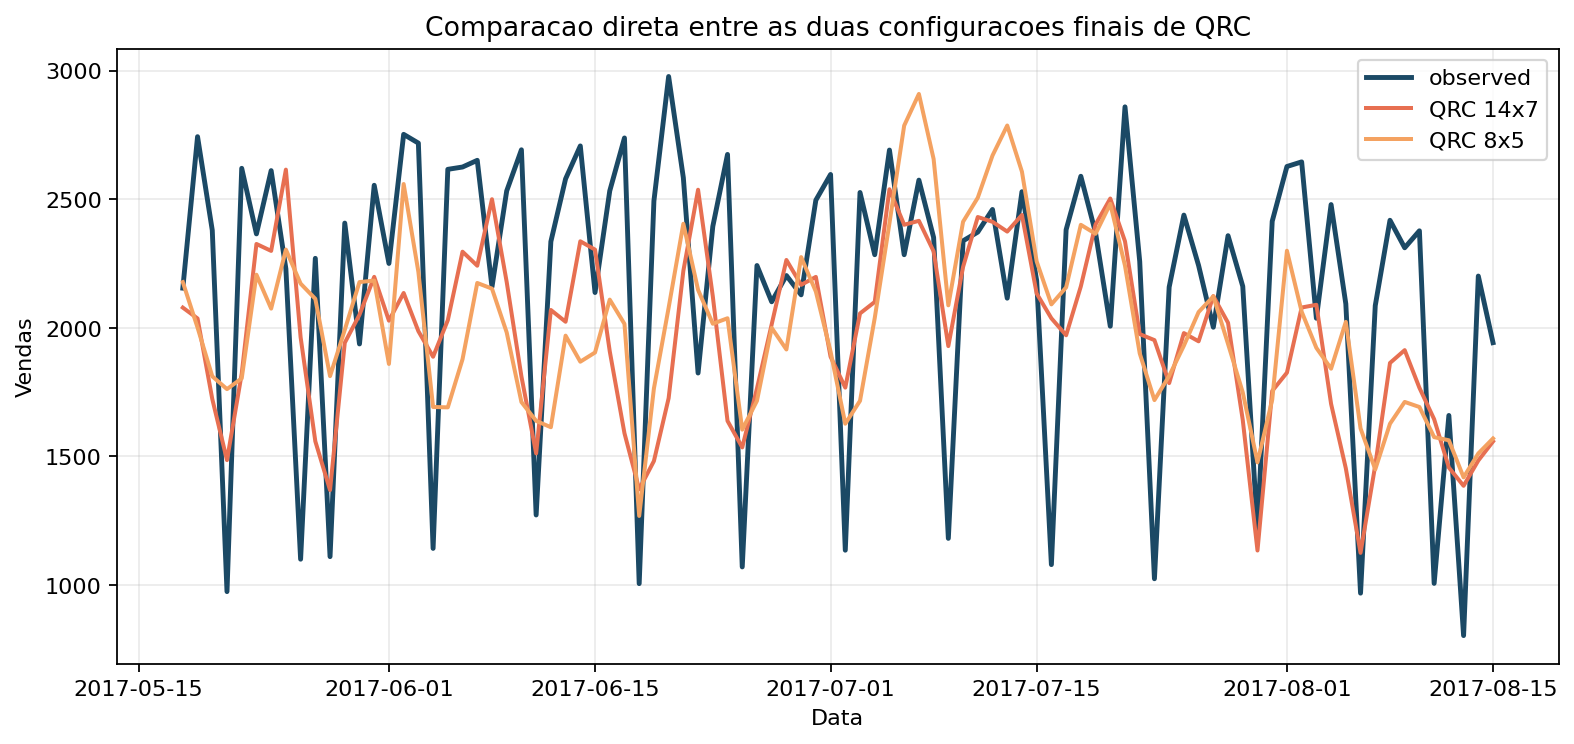
\includegraphics[keepaspectratio,alt={Comparação direta entre as configurações QRC14x7 e QRC8x5.}]{computational_results_20260402_222902/qrc_14x7_vs_8x5.png}}

\pandocbounded{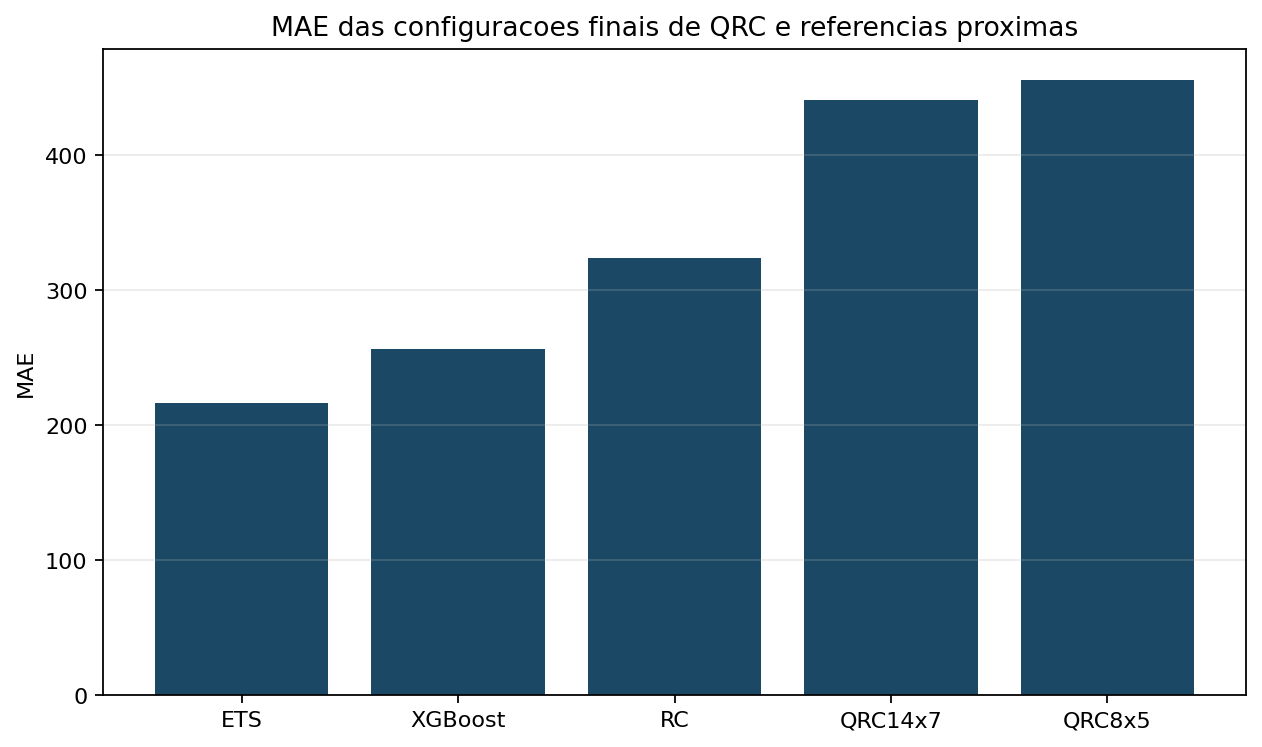
\includegraphics[keepaspectratio,alt={Comparação em barras para o MAE entre modelos de referencia e QRC.}]{computational_results_20260402_222902/qrc_focus_mae_bars.png}}

A leitura dos dois pontos é clara:

\begin{itemize}
\tightlist
\item
  \texttt{14x7} foi melhor que \texttt{8x5} nas quatro métricas no run direto;
\item
  \texttt{8x5} permaneceu relevante porque sua função objetivo penalizada era melhor;
\item
  o trade-off entre desempenho e complexidade foi real, não artificial.
\end{itemize}

\subsection{7. Comparação com RC e técnicas clássicas}\label{7-comparauxe7uxe3o-com-rc-e-tuxe9cnicas-cluxe1ssicas}

O QRC precisa ser lido ao lado do benchmark herdado, não isoladamente.

\begin{longtable}[]{@{}lllll@{}}
\toprule\noalign{}
Modelo & MAE & RMSE & WAPE & sMAPE \\
\midrule\noalign{}
\endhead
\bottomrule\noalign{}
\endlastfoot
ETS & 216.303 & 307.638 & 0.0999 & 0.1042 \\
XGBoost & 256.666 & 332.828 & 0.1185 & 0.1237 \\
RC & 324.294 & 423.417 & 0.1498 & 0.1653 \\
QRC14x7 & 441.286 & 525.325 & 0.2038 & 0.2269 \\
QRC8x5 & 455.833 & 526.949 & 0.2105 & 0.2342 \\
\end{longtable}

O ponto central do estudo e este:

\begin{itemize}
\tightlist
\item
  \texttt{QRC14x7} ficou cerca de 36.1\% acima do \texttt{RC} em \texttt{MAE};
\item
  \texttt{QRC14x7} ficou cerca de 104.0\% acima do \texttt{ETS} em \texttt{MAE};
\item
  ainda assim, o pipeline quântico funcionou de ponta a ponta no mesmo recorte de negócio.
\end{itemize}

\subsection{8. O que os resultados mostram e o que eles não mostram}\label{8-o-que-os-resultados-mostram-e-o-que-eles-nuxe3o-mostram}

\subsubsection{8.1 O que mostram}\label{81-o-que-mostram}

\begin{itemize}
\tightlist
\item
  QRC pode ser implementado de modo didático e reprodutivel com Qiskit;
\item
  tuning de \texttt{qubits} e \texttt{window} importa muito;
\item
  o melhor QRC do projeto foi \texttt{14x7};
\item
  comparações honestas sao possíveis no mesmo recorte adotado no Favorita.
\end{itemize}

\subsubsection{8.2 O que não mostram}\label{82-o-que-nuxe3o-mostram}

\begin{itemize}
\tightlist
\item
  que QRC seja superior a técnicas clássicas neste problema;
\item
  que aumentar qubits sempre melhora desempenho;
\item
  que o estudo atual esgote o espaco de arquiteturas quânticas possíveis.
\end{itemize}

\subsection{9. A contribuição didática do estudo final}\label{9-a-contribuiuxe7uxe3o-diduxe1tica-do-estudo-final}

O estudo final não vale apenas pela tabela de métricas. Ele vale porque fecha uma trilha de ensino completa:

\begin{enumerate}
\def\labelenumi{\arabic{enumi}.}
\tightlist
\item
  do problema de negócio;
\item
  aos baselines;
\item
  ao RC clássico;
\item
  ao tuning;
\item
  ao benchmark justo;
\item
  a ponte quântica;
\item
  ao QRC implementado e comparado.
\end{enumerate}

Essa sequência e o que transforma o conjunto dos sete artigos em um material "101" real para QRC.

\subsection{10. O que o leitor aprendeu do artigo 1 ao 7}\label{10-o-que-o-leitor-aprendeu-do-artigo-1-ao-7}

Ao final da série, o leitor passou a saber:

\begin{itemize}
\tightlist
\item
  formular um problema real de previsão de demanda;
\item
  construir um protocolo temporal correto;
\item
  comparar baselines, IA clássica, RC e QRC;
\item
  ler e modificar as implementações do projeto;
\item
  interpretar resultados negativos ou medianos sem perder valor científico;
\item
  entender QRC como extensão do paradigma de reservatório, e não como curiosidade isolada.
\end{itemize}

\subsection{11. Conclusão}\label{11-conclusuxe3o}

O QRC do projeto funciona, ensina, compara e fecha a série de forma honesta. O melhor resultado puro ficou em \texttt{14x7}; o melhor compromisso com penalizacao de complexidade ficou em \texttt{8x5}. Nenhum dos dois venceu os melhores modelos clássicos no recorte adotado no Favorita, mas ambos cumprem o papel mais importante desta obra: ensinar, de forma continua e reproduzível, como sair do zero e chegar a um estudo completo de Quantum Reservoir Computing aplicado a um problema real.

\subsection{Entregaveis associados no repositorio}\label{entregaveis-associados-no-repositorio}

\begin{itemize}
\tightlist
\item
  implementação do QRC: \texttt{code/qrc/}
\item
  tuning e função objetivo: \texttt{code/qrc/objective.py}, \texttt{code/qrc/OBJECTIVE.md}
\item
  benchmark consolidado: \texttt{code/RESULTS.md}
\item
  artefatos deste artigo: \texttt{computational\_results\_20260402\_222902/}
\end{itemize}

\subsection{Referencias}\label{referencias}

\begin{itemize}
\tightlist
\item
  Fujii, K.; Nakajima, K. Harnessing disordered-ensemble quantum dynamics for machine learning.
\item
  Ghosh, S. et al. Quantum reservoir processing.
\item
  Qiskit documentation.
\item
  Jaeger, H. The "echo state" approach to analysing and training recurrent neural networks.
\item
  Monzani, F.; Ricci, E.; Nigro, L.; Prati, E. QRC-Lab: An Educational Toolbox for Quantum Reservoir Computing. arXiv:2602.03522.
\end{itemize}

        \end{document}
